\documentclass[25pt, a0paper, portrait, margin=0mm, innermargin=20mm,
blockverticalspace=2mm, colspace=20mm, subcolspace=0mm]{tikzposter} %Default values for poster format options.

\usepackage[utf8]{inputenc}
\usepackage[scaled]{helvet}
\renewcommand\familydefault{\sfdefault} 
\usepackage[T1]{fontenc}
\usepackage{wrapfig}
\usepackage{setspace}
\usepackage{multicol}
\setlength{\columnsep}{1.5cm}
\usepackage{xspace}
\usepackage{tikz}
\tikzposterlatexaffectionproofoff
\usetheme{Default}

\definecolor{unired}{HTML}{a51e37}
\definecolor{mypink1}{rgb}{0.858, 0.188, 0.478}
\definecolor{mblack}{HTML}{0d0d0d}
\definecolor{titlecolor}{RGB}{74, 114, 159}
\definecolor{titledarkcolor}{RGB}{51,102,153}
\definecolor{Grey}{HTML}{e1e1e1}
\definecolor{DarkerGrey}{RGB}{215,217,219}
\definecolor{FontColor}{HTML}{0d0d0d}
\definecolor{Red}{RGB}{204,0,0}
\definecolor{L-lig}{RGB}{25,124,192}
\definecolor{point-lig}{RGB}{255,255,255}
\definecolor{G-lig}{RGB}{62,66,68}

\definecolor{Orange}{RGB}{240,163,10} 
\definecolor{LightRed}{RGB}{214,98,93}
\definecolor{LightBlue}{RGB}{160,200,217}
\definecolor{LightGreen}{RGB}{130,161,119}
\definecolor{Violet}{RGB}{190,144,252}

\colorlet{blocktitlefgcolor}{mblack}
\colorlet{backgroundcolor}{Grey}
\colorlet{blocktitlebgcolor}{Grey}
\colorlet{blockbodyfgcolor}{FontColor}
\colorlet{innerblocktitlebgcolor}{L-lig}
\colorlet{innerblocktitlefgcolor}{white}
\colorlet{notefrcolor}{white}
\colorlet{notefgcolor}{black}
\colorlet{notebgcolor}{white}


% Title setup
\settitle{ 
\begin{minipage}[b]{0.8\linewidth}
\vspace{2cm}
\hspace{1cm}\color{mblack}{ \Huge{\textbf{\@title}} \par } \vspace*{2em} \hspace{1cm}\color{mblack}{\LARGE \@author \par} \vspace*{2em} \hspace{1cm}{\Large \@institute}\vspace{0.5cm} \end{minipage}

% Add institution logo
\hfill
\begin{minipage}[t]{0.2\linewidth}
    \vspace{-13.8cm}\hspace{-3.8cm}
    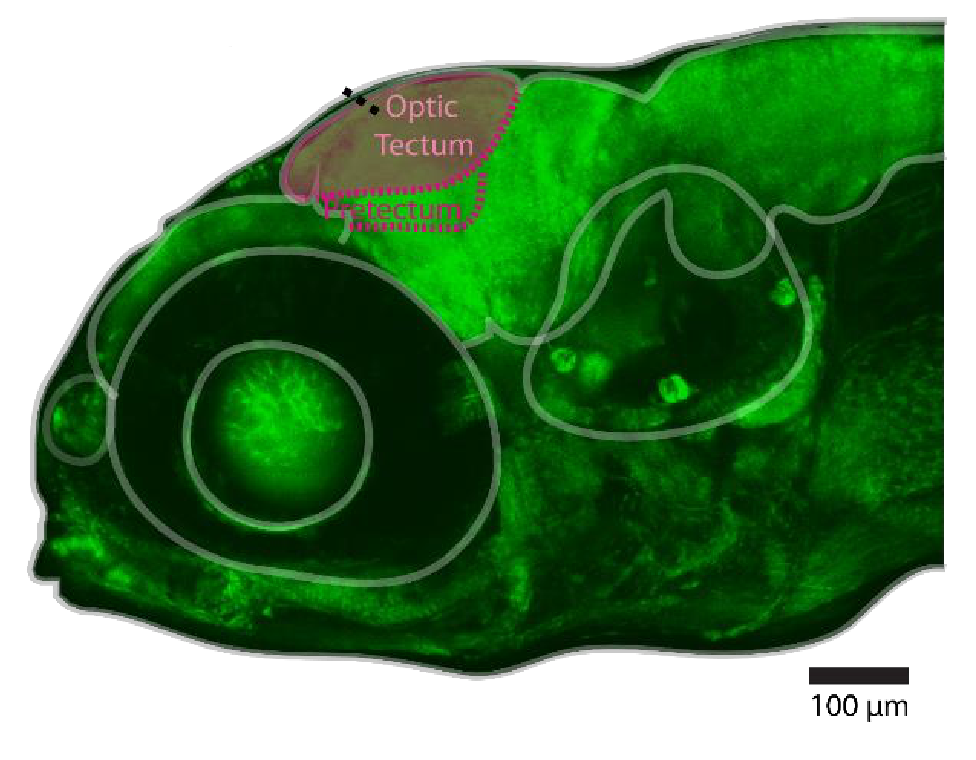
\includegraphics[width=13cm]{figs/titlepic.png} 
\end{minipage}}

% define title style with background box (currently white)
\definetitlestyle{sampletitle}{
width=841mm, roundedcorners=0, linewidth=0pt, innersep=15pt,
titletotopverticalspace=0mm, titletoblockverticalspace=5pt
}{\begin{scope}[line width=\titlelinewidth, rounded corners=\titleroundedcorners]\draw[fill=point-lig, color=point-lig]
(\titleposleft,\titleposbottom) rectangle (\titleposright,\titlepostop);
\end{scope}}

 % Title, Author, Institute
\title{\parbox{1500pt}{Complex frequency modulations in freely interacting electric fish, \textit{Apteronotus leptorynchus}, recorded in their natural habitat}}
\author{Patrick Weygoldt, Till Raab, Jan Benda}
\institute{Neuroethology Lab, Department of Neurobiology, University of Tuebingen}
\usetitlestyle[]{sampletitle}

% define coustom block style
\defineblockstyle{MyBlock}{% define a custom style for a block
    titlewidthscale=1, bodywidthscale=1, titlecenter,
    titleoffsetx=0pt, titleoffsety=-30pt, bodyoffsetx=0pt, bodyoffsety=-40pt,
    bodyverticalshift=0mm, roundedcorners=25, linewidth=1pt,
    titleinnersep=20pt, bodyinnersep=38pt
}{
    \draw[rounded corners=\blockroundedcorners, inner sep=\blockbodyinnersep,
          line width=\blocklinewidth, color=white,
          top color=titlebgcolor!90, bottom color=titlebgcolor!20!white,
          ]
      (blockbody.south west) rectangle (blockbody.north east); %
    \ifBlockHasTitle%
        \draw[rounded corners=\blockroundedcorners, inner sep=\blocktitleinnersep,
          top color=Grey, bottom color=Grey,
          line width=2, color=Grey, %fill=blocktitlebgcolor
          ]
      (blocktitle.south west) rectangle (blocktitle.north east); %
    \fi%
}
\newcommand\myblock[3][MyBlock]{\useblockstyle{#1}\block{#2}{#3}\useblockstyle{Default}}

\begin{document}
 
\renewcommand{\baselinestretch}{1} 
\title{\parbox{1500pt}{Color-blindness of direction-selective units in the \\ zebrafish optic tectum}}
\author{Alexander Wendt, Patrick Weygoldt}
\institute{Supervisor: Aristides Arrenberg, Tim Hladnik, David Burkhardt}
\usetitlestyle[]{sampletitle}
\maketitle
\renewcommand{\baselinestretch}{1.4} 

\begin{columns}
\column{0.3333}
\myblock[MyBlock]{Introduction}{
    Orger and Baier (2004) demonstrated that chromaticity has a big influence on a zebrafishs ability to perceive motion. 
    The optomotor response to gratings showed that combinations of different green and red contrasts can be used to null motion perception.
    \vspace{0.7cm}
    \begin{tikzfigure}[]
    \label{Raw}
    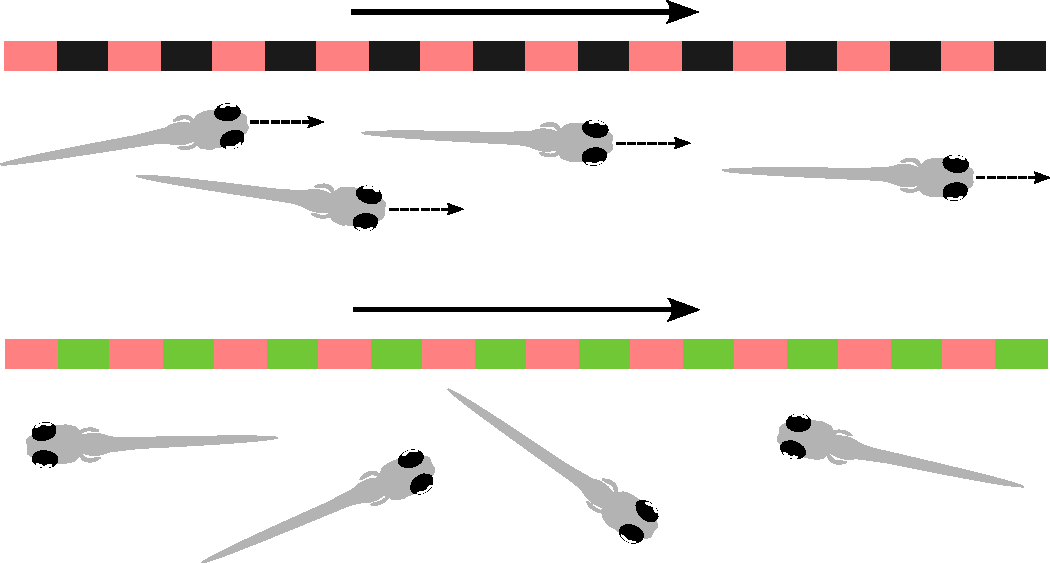
\includegraphics[width=17cm]{figs/omr.pdf}
    \end{tikzfigure} 
   
   Little is known about the sensitivity of direction selective (ds) units in the midbrain to chromatic contrast. We investigated the 
   activity of ds units in the optic tectum of zebrafish in response to gratings of various color contrasts using a combination of two-photon microscopy and calcium imaging. 
}
\myblock[MyBlock]{Preprocessing:}{
    \textbf{1. Registration and Segmentation}
    \begin{tikzfigure}[]
        \label{Rois}
        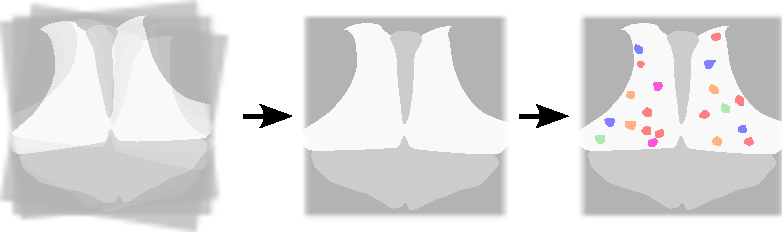
\includegraphics[width=22cm]{figs/drawing.pdf} 
    \end{tikzfigure}

    \begin{itemize}
        \item Alignment of images across time.
        \item Detection and segmentations to regions of interests (ROIs).
    \end{itemize}

    \textbf{2. Region of Interests (ROI):}
    corresponds to cells with genetically encoded calcium indicators. 
    Fluorescence increases with the release of calcium in a cell if excited by a IR-laser.
    
    % An ROIs fluorescence $F$ is calculated from the change of fluorescence normalized to the average fluorescence $F = \frac{F - \langle F \rangle}{\langle F \rangle}$.
    
    \vspace{0.5cm}
    \begin{tikzfigure}[]
        \label{Raw}
        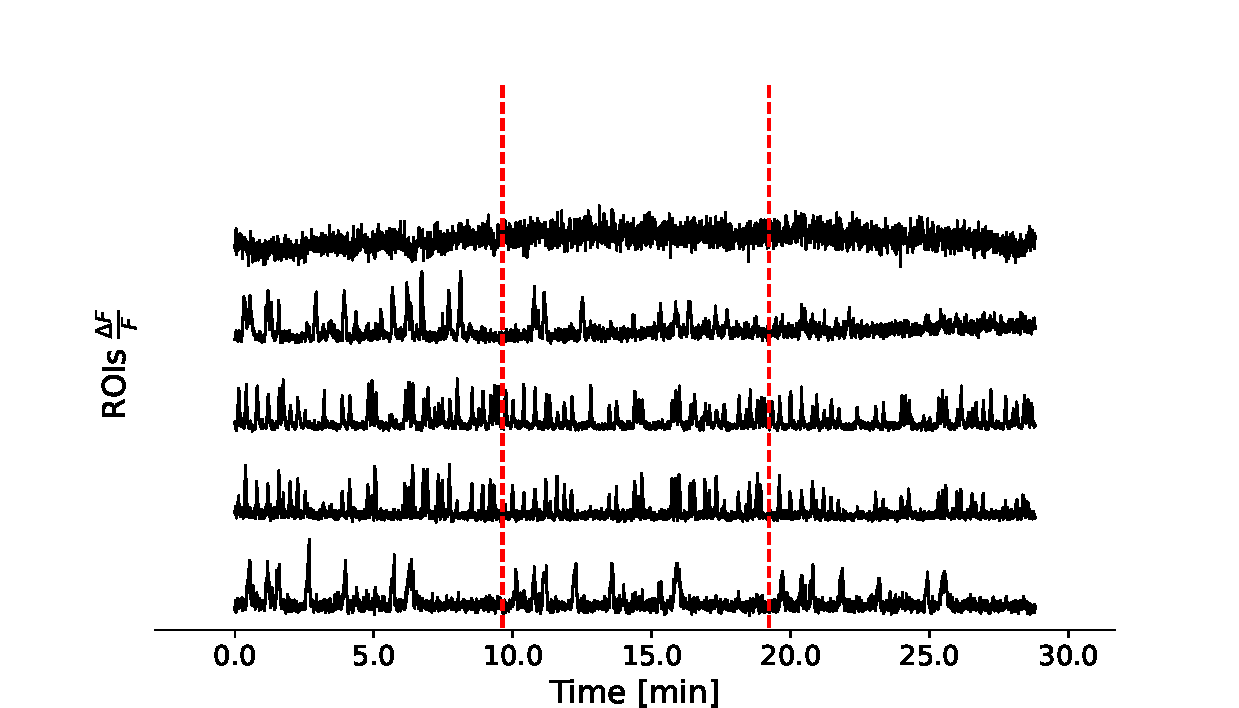
\includegraphics[width=22cm]{figs/autocorrelation.pdf}
    \end{tikzfigure} 
    \vspace{0.6cm}
    \textbf{3. Active and direction-selective ROIs:} 
    \begin{itemize}
        \item Strongly autocorrelated ROIs across stimulus repeats are \glqq responding\grqq{}.
        \item ROIs that correlated with a direction regressor (clockwise cw or counterclockwise ccw) are ds.
    \end{itemize}
    \begin{tikzfigure}[]
        \label{Rois}
        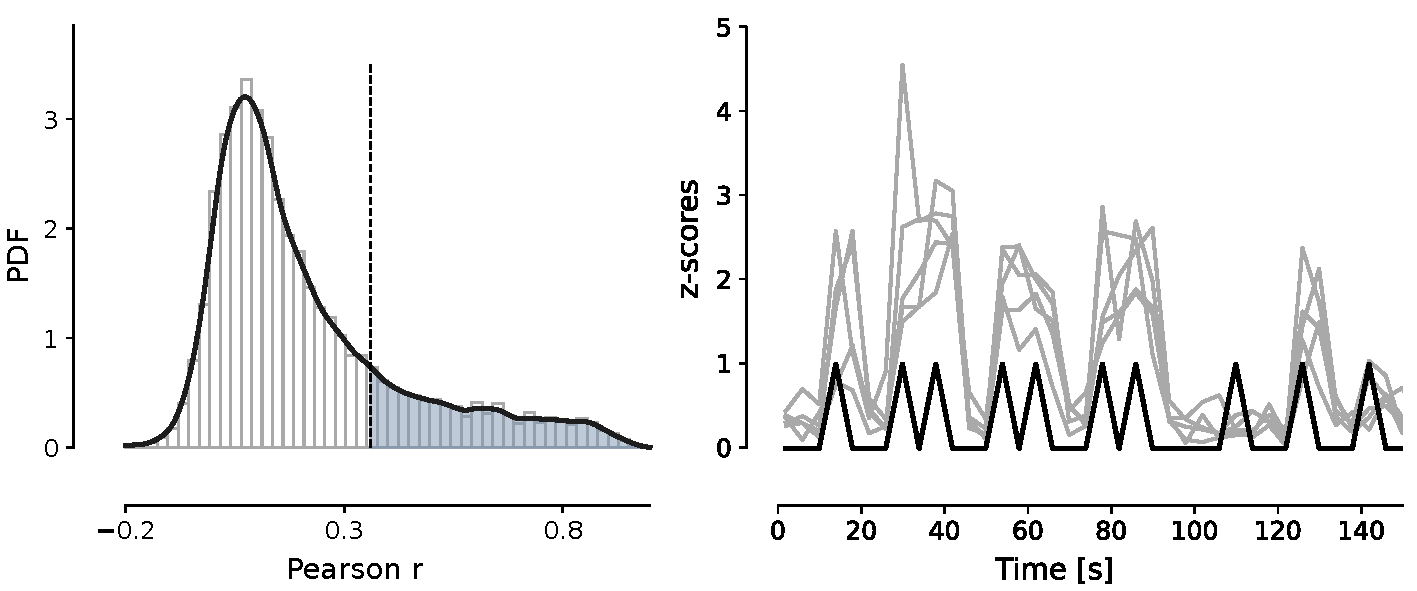
\includegraphics[width=22cm]{figs/pcorrelation.pdf} 
    \end{tikzfigure}
    \vspace{0.5}
    
    % \vspace{-1.3cm}
    % \begin{tikzfigure}[]
    %     \label{Rois}
    %     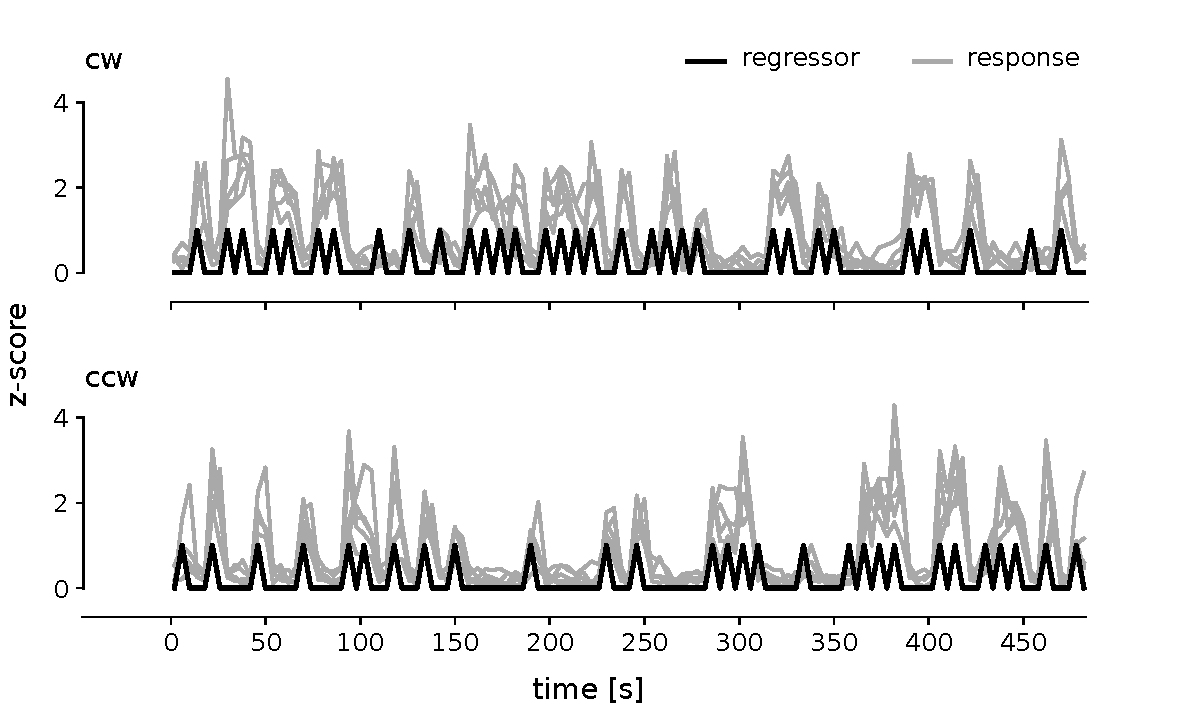
\includegraphics[width=24cm]{figs/regressor.pdf}
    % \end{tikzfigure}
}  
\column{0.6666}
\myblock[MyBlock]{Results: 2-photon calcium imaging}{
    \vspace{-1.7cm}
    \begin{tikzfigure}[]
        \label{modulations}
        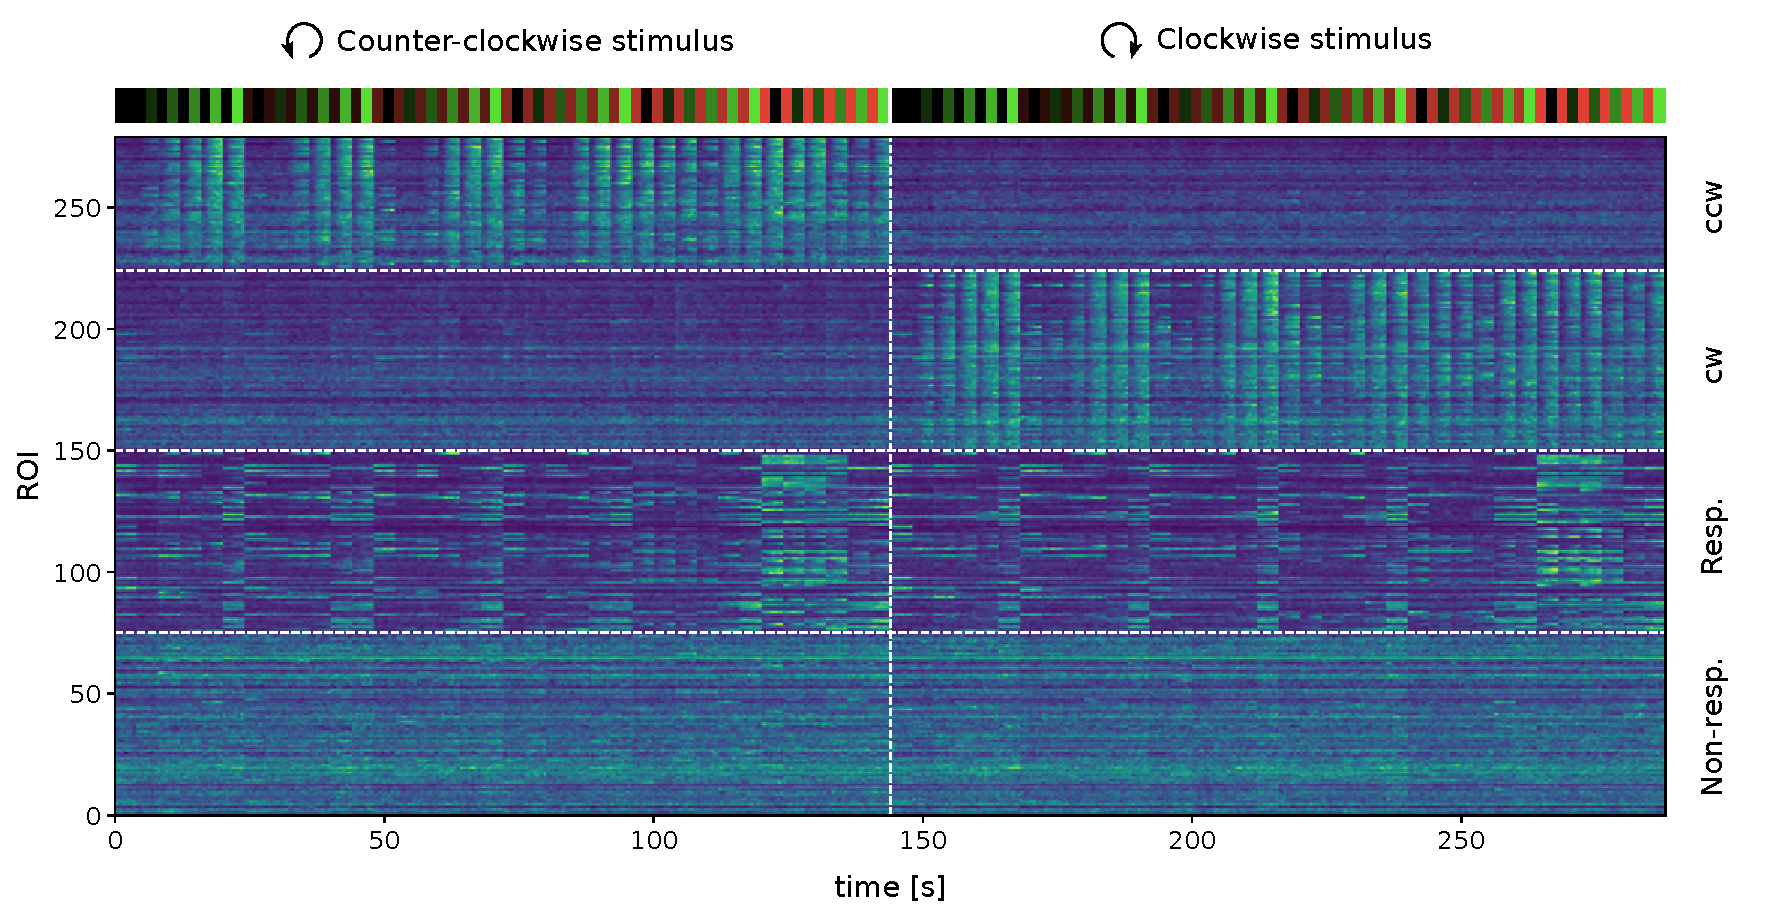
\includegraphics[width=\linewidth]{figs/testimg.pdf
        }
    \end{tikzfigure}

    \begin{tikzfigure}[]
        \label{Raw}
        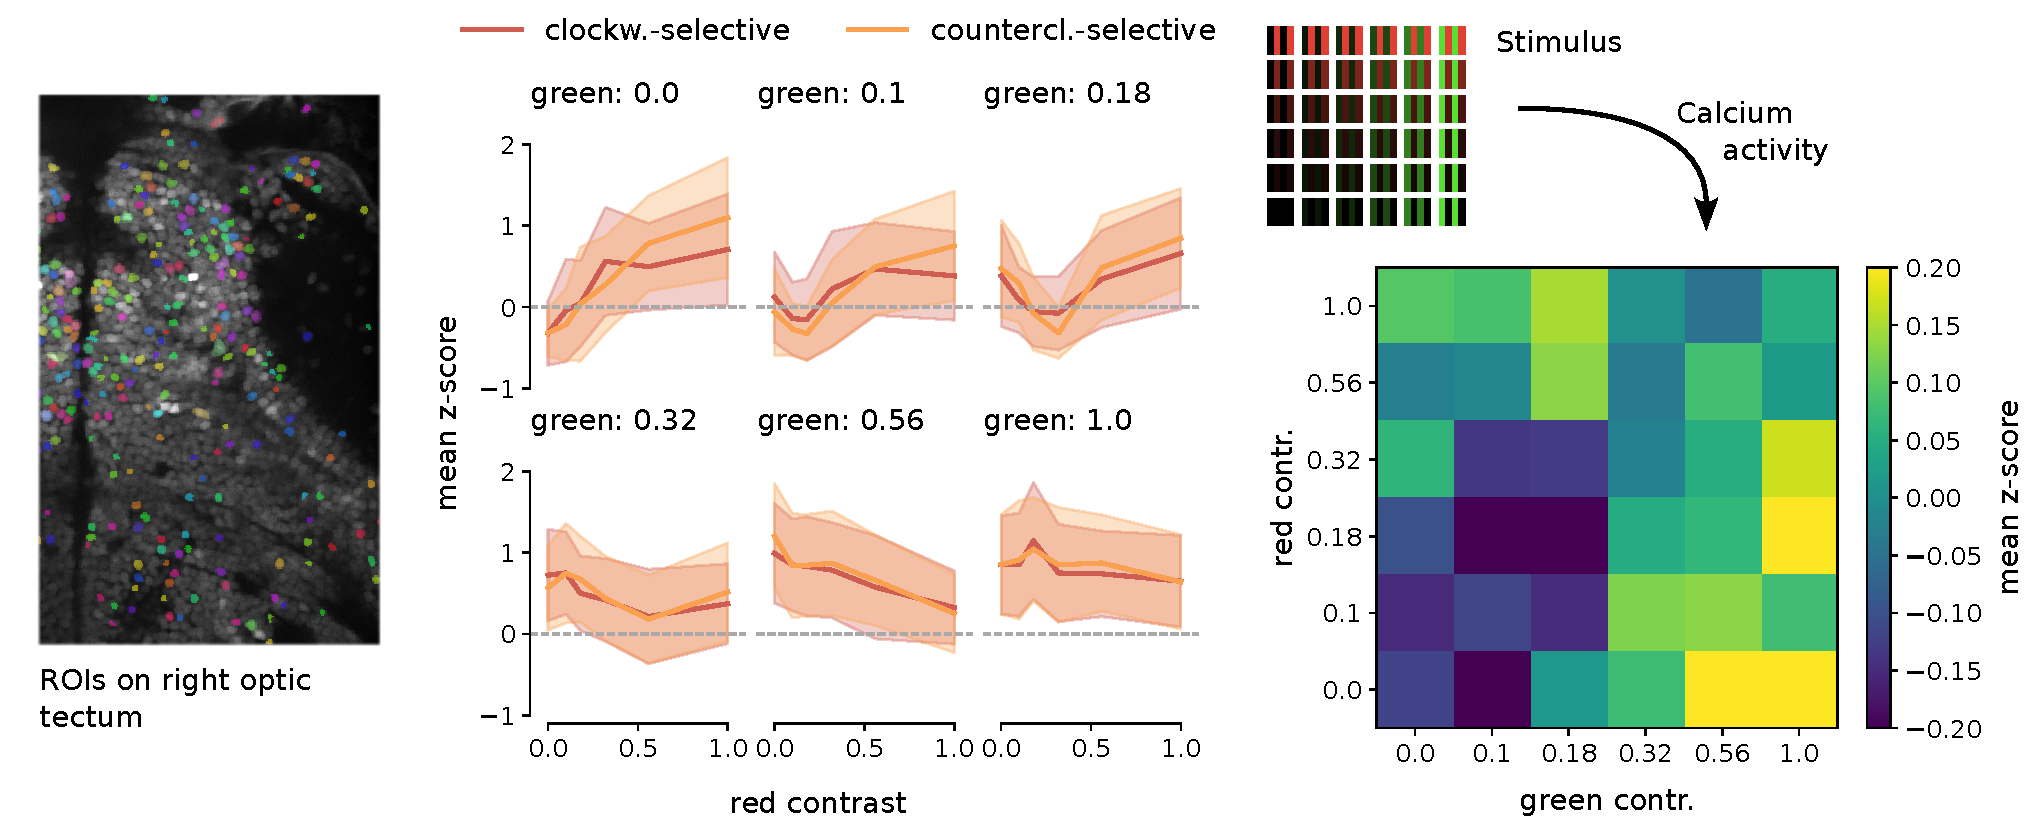
\includegraphics[width=50cm]{figs/contrast_curves_ca.pdf}
    \end{tikzfigure}

    \begin{itemize}
        \item ROIs responded to moving gratings of red and green and both populations (cw, ccw) responded similarly.
        \item If both red and green had the same contrast the response was supressed indicating color blindness of direction selective units.
        \item A slight shift in the troughs of activity could be due to by a higher intensity of the green stimulus compared to red.
    \end{itemize}
}   
\myblock[MyBlock]{Results: Behavior}{
    \vspace{-1.7cm}
    \begin{tikzfigure}[]
        \label{Raw}
        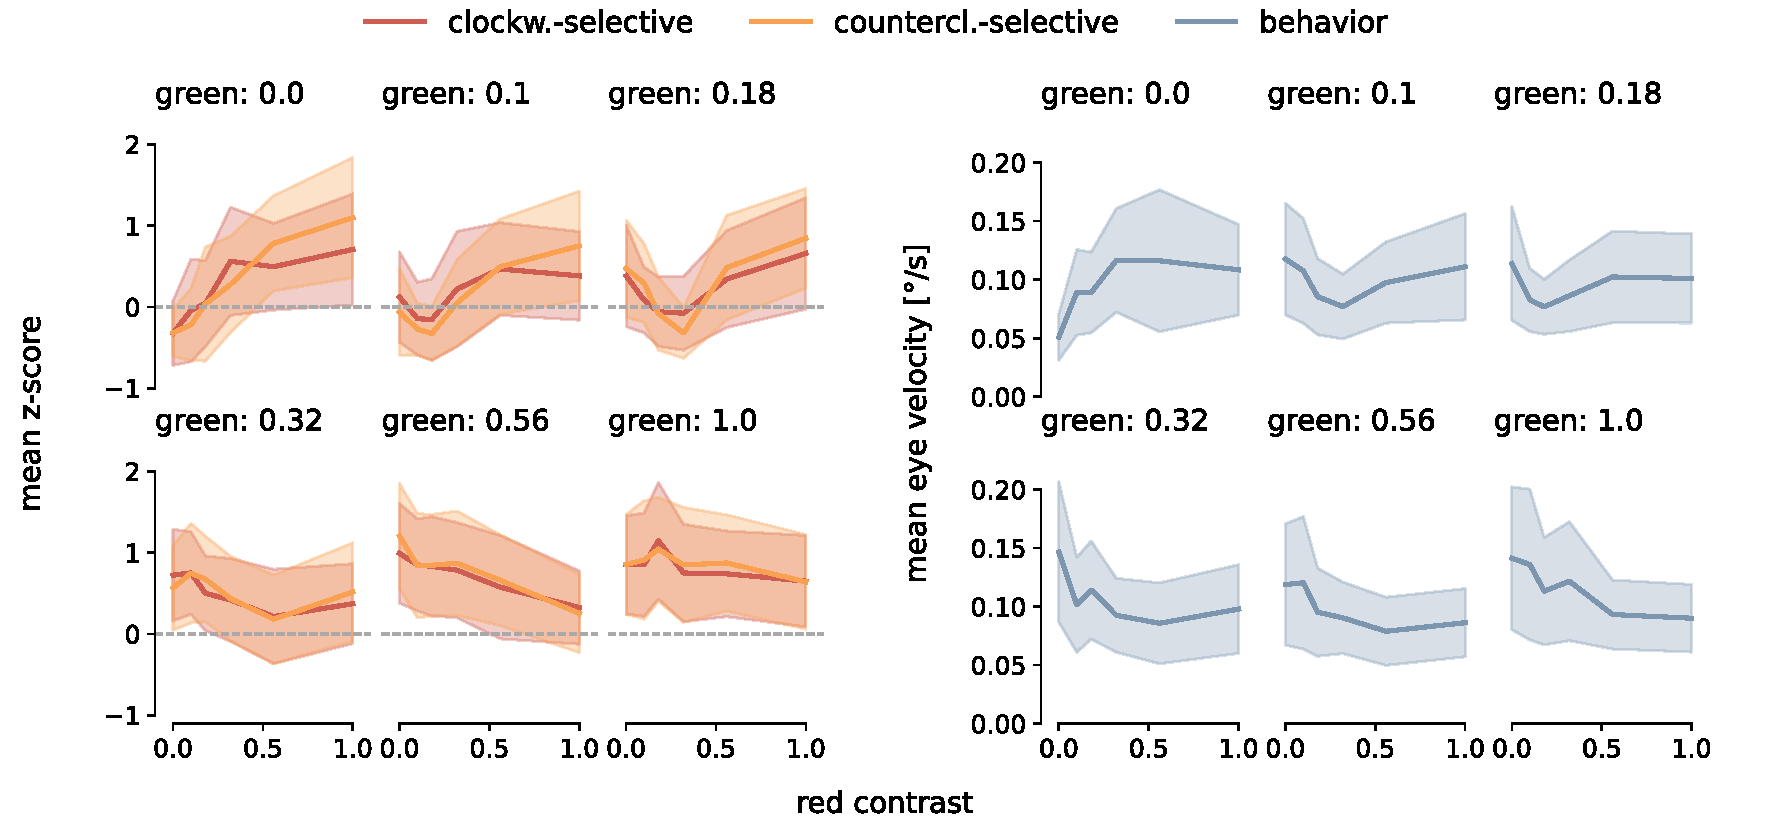
\includegraphics[width=50cm]{figs/contrast_curves_behav_test.pdf}
    \end{tikzfigure}
    \begin{itemize}
        \item The behavioral response (OKR) reflects the pattern shown in calcium activity.
    \end{itemize}
}
\myblock[MyBlock]{Conclusion}{
        \setlength\itemsep{0.5cm}
        The ds neurons in the optic tectum show the lowest response to exclusively chromatic red-green contrast and might therefore be color blind to these contrasts.
    \vspace{0.2cm}
    }
\end{columns}

\node [above right, text=white, outer sep=45pt,minimum width=\paperwidth, align=center, draw, fill=unired, color=unired] at (-43.6,-61) { \textcolor{white}{\normalsize Contact: surname.name@student.uni-tuebingen.de}};

\end{document}